\chapter{Multi Language App}

After building support for various languages and their interaction in previous sections, this section demonstrates how to build a real world application using multiple languages. For this project, we created hotel search application which takes advantages of multi-language environment to render the app. This application helps user to search for hotels by specifying the city and country. 

Apart from taking advantage of multi-language environment (Scheme, Lua, and JavaScript), app also uses libraries like "Google maps APIs" \cite{googlemapsapi}, "Jquery" \cite{jquery} etc. Home screen of the application is shown in Figure \ref{fig:multilangapp}.

\begin{figure}[H]
	\begin{center}
		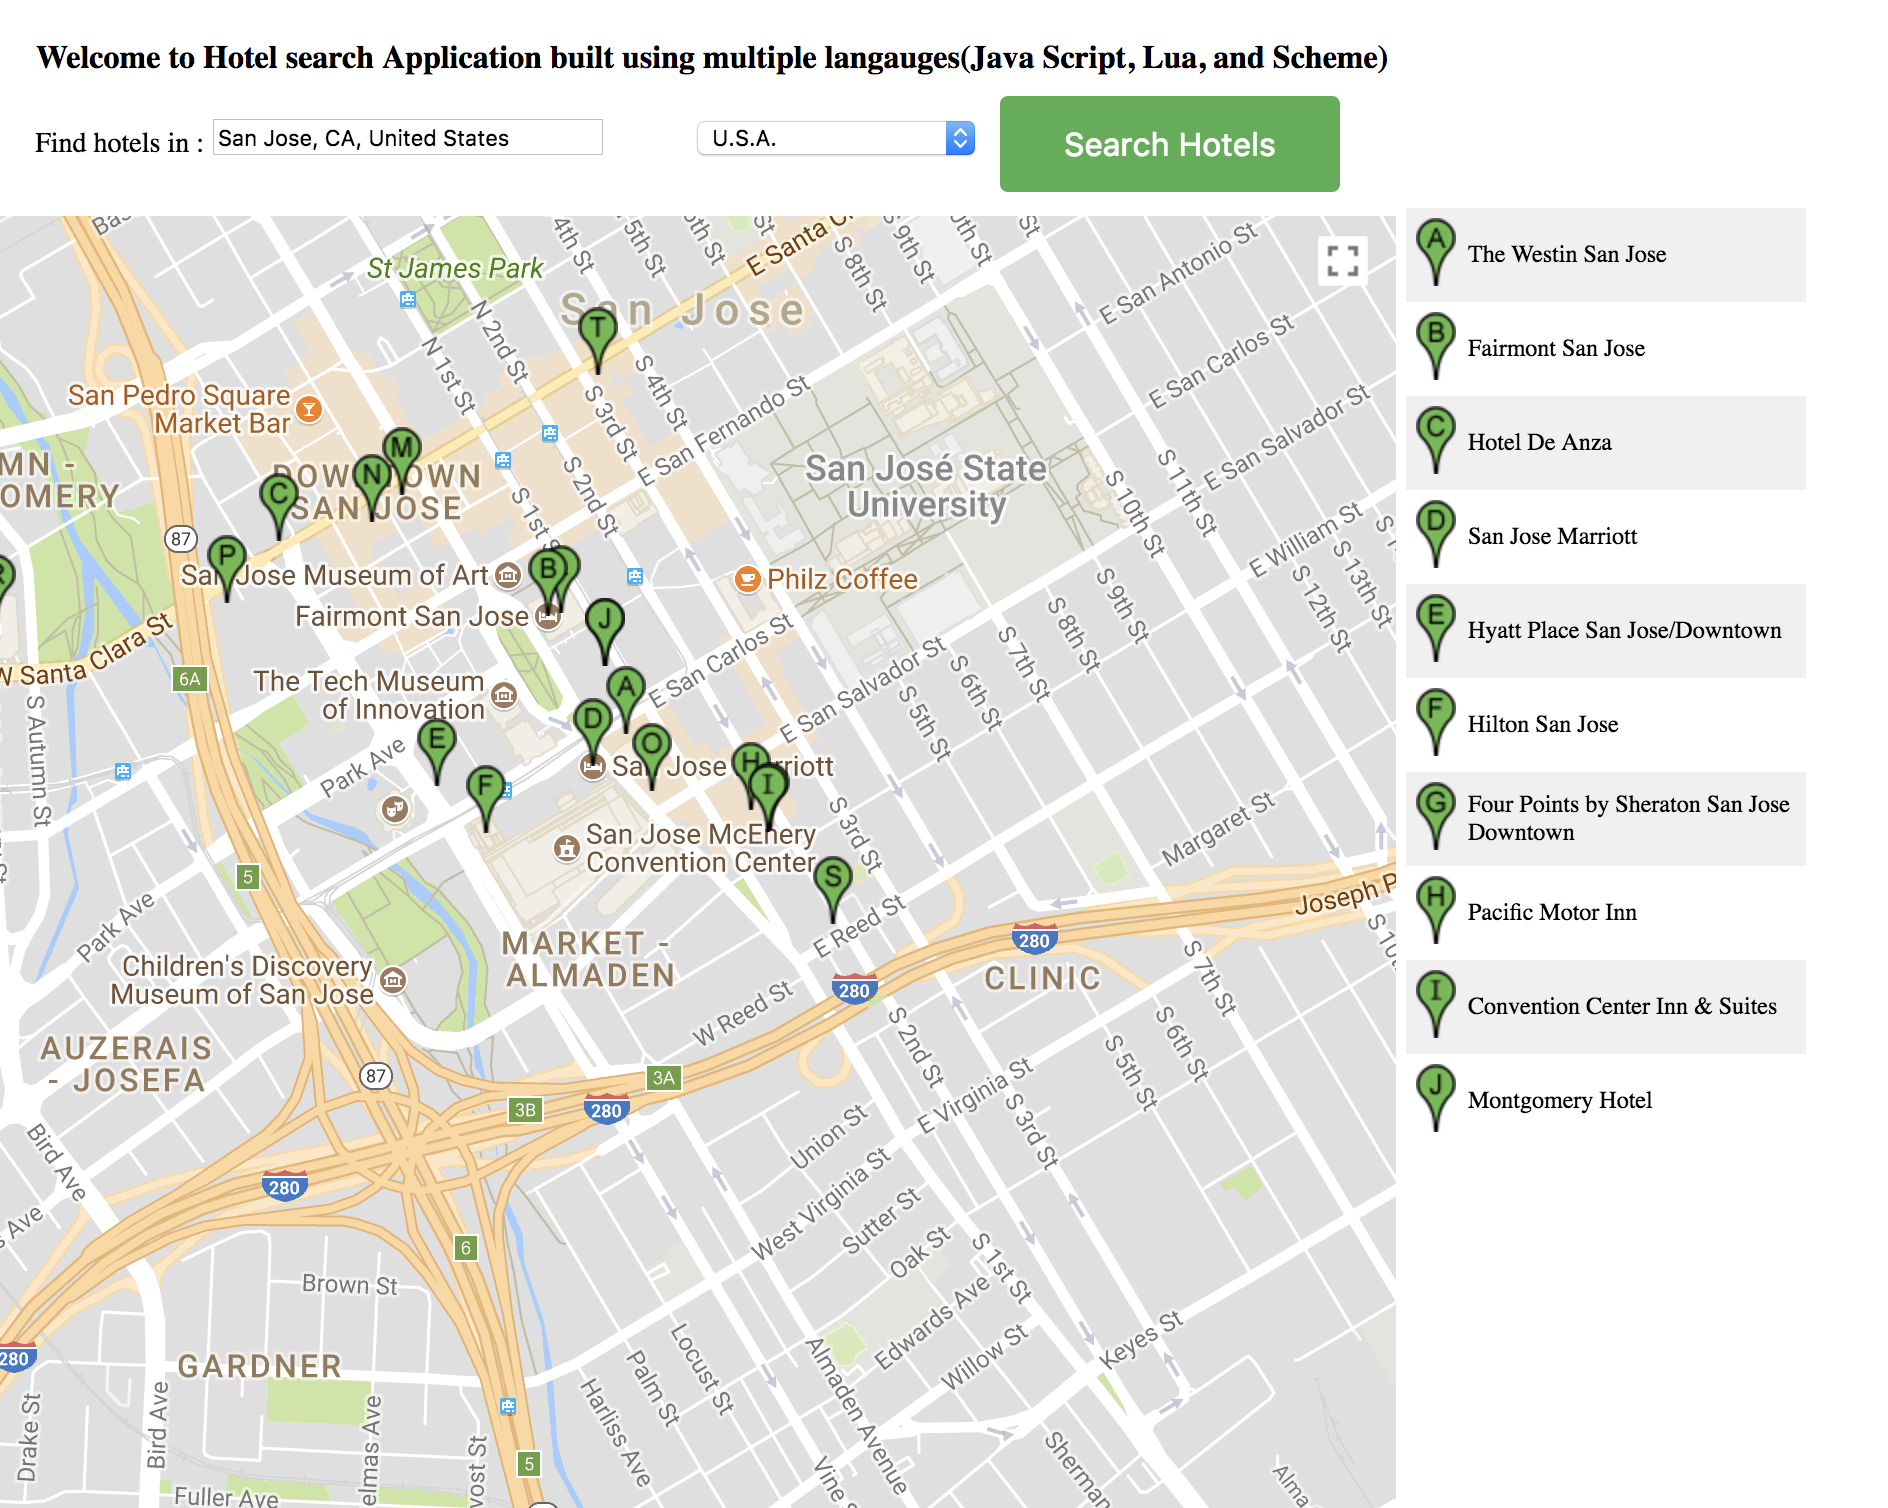
\includegraphics[width=\linewidth]{./images/multilangapp.png}
	\end{center}
	\caption{Hotel Search: Multi-language Application}
	\label{fig:multilangapp}
\end{figure}

Application provides the following functionalities : 
\begin{itemize}
	\item {\textbf{Cities Auto Complete} : It provides the interface to enter the city. }
	\item {\textbf{Country Drop Down} : It provides the drop down to select the countries from a list of countries.}
	\item {\textbf{Search Button} : Button to search hotels in a selected city.}
	\item {\textbf{Map} : Provides a window to display google map on the screen.}
	\item {\textbf{Result} : Provides a content holder to show the search results.}
\end{itemize}

JavaScript in the application handles rendering of the map and fetching search result from google places API. JavaScript maintains the reference to maps, countries selected, search text in its global scope. JavaScript also calls Scheme's "getElem" function to get the reference of particular element on the page, as shown in Figure \ref{fig:js-code}, 

\begin{figure}[H]
	\begin{lstlisting}
	
	// Gets the map element reference.
	var elem =scheme.evaluate(`(getelem "#map")');
	
	// Gets the Result window reference.
	var infocontent = scheme.evaluate(`(getelem ``#info-content'')');
	
	// Gets the Search City text box reference.
	var autocomplet = scheme.evaluate(`(getelem '``#autocomplete'')');
	
	\end{lstlisting} 
	\caption{JavaScript code}
	\label{fig:js-code}
\end{figure}


Scheme code in the application is responsible for initializing the app, and provide on click functionality for the "Search Hotels" button, as shown in Figure \ref{fig:schemeINteraction}.

\begin{figure}[H]
	\begin{center}
		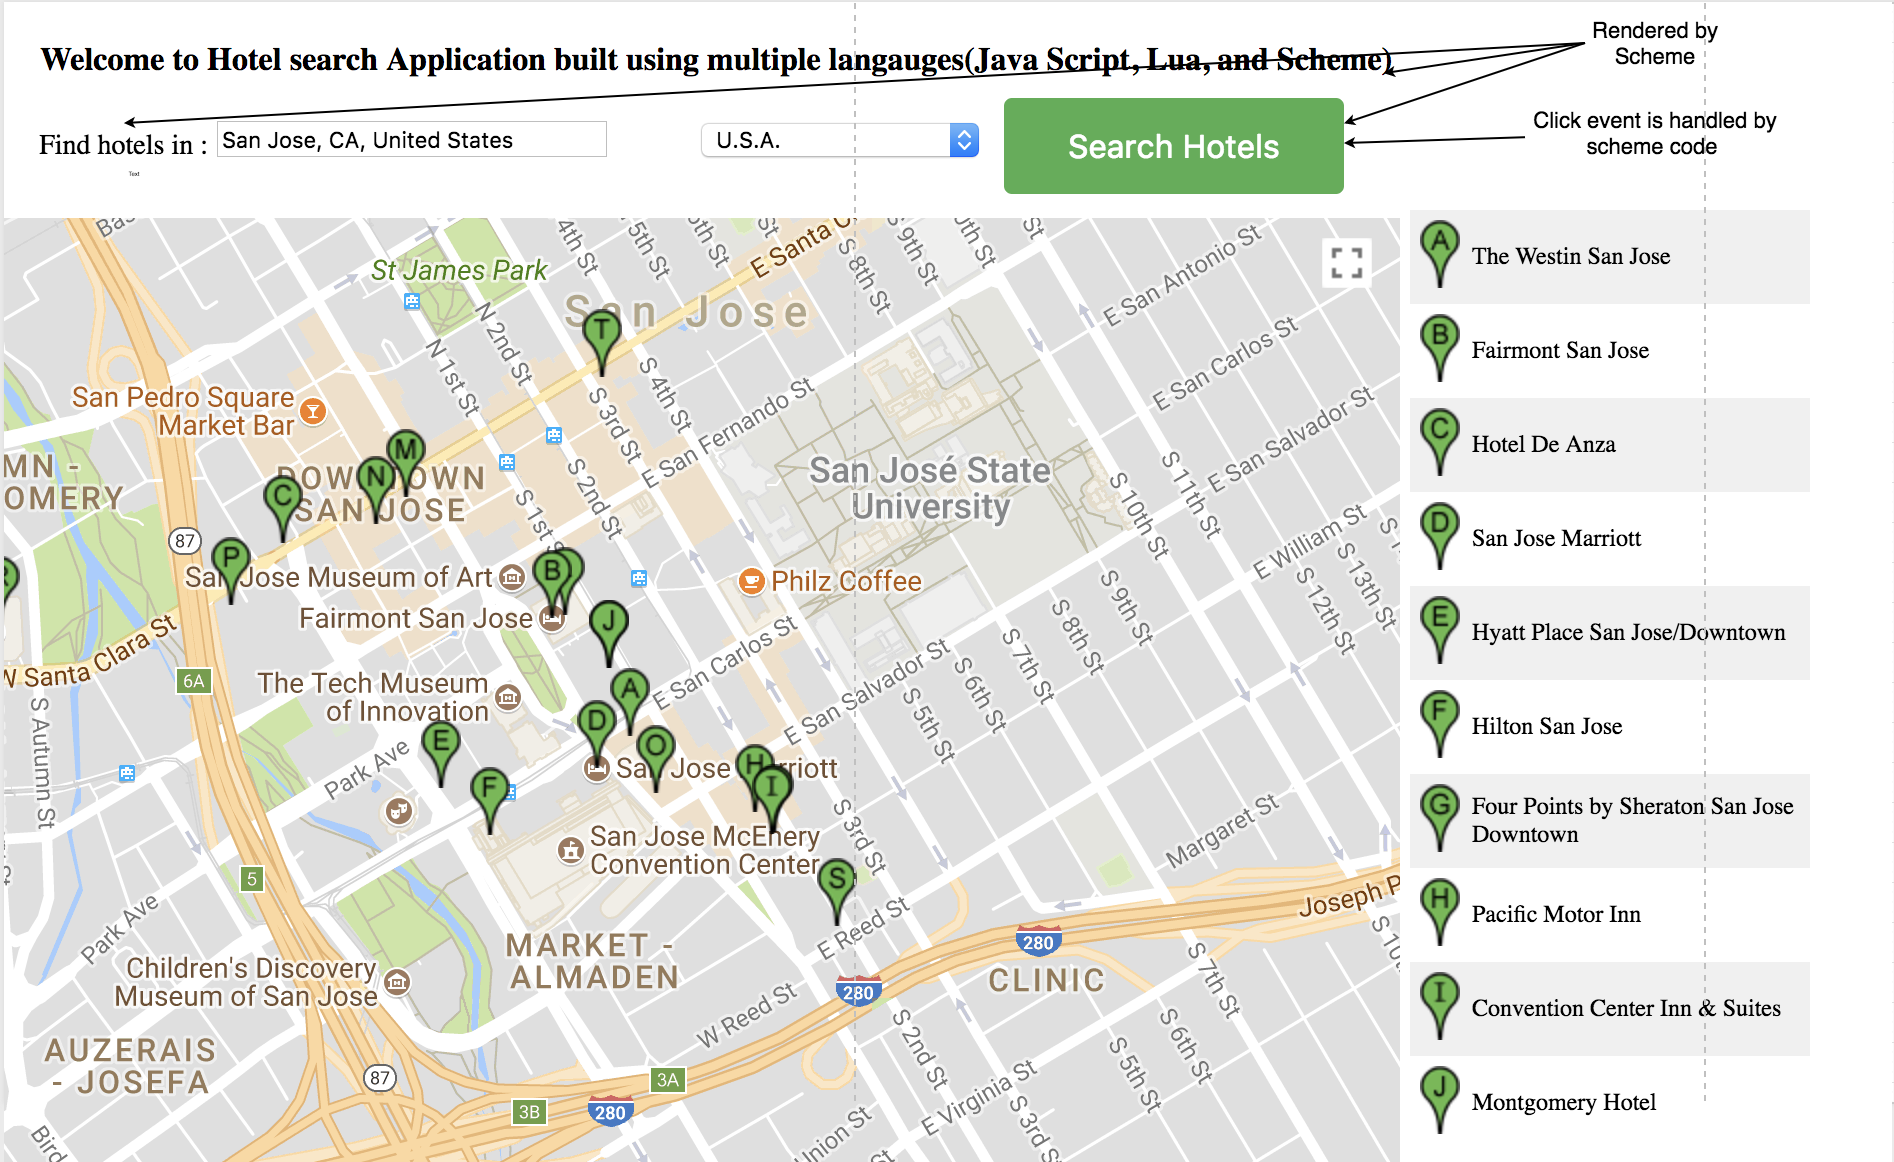
\includegraphics[width=\linewidth]{./images/schemeINteraction.png}
	\end{center}
	\caption{Scheme Contribution: Hotel Search Application}
	\label{fig:schemeINteraction}
\end{figure}

Following code shows the scheme code which enable the functionalities shown in figure \ref{fig:schemeINteraction}

 \begin{lstlisting}[frame=single, style=base]
<script type="text/scheme">
(
  ;;; Logs welcome message
  (console-log "Welcome !!!")
 
 ;;; Declare InitialiseApplication function 
 ;;; which initialisation the app
 (define initialiseApplication
 (lambda ()
  
  ;;; Updates the Header text to specified string
  (element-update! "#header" "Welcome to Hotel search 
   Application built using multiple langauges
   (Java Script, Lua, and Scheme)")
  
   ;;; Updates the Search Button text to specified string
  (element-update! "#searchButton" "Search Hotels")
  
   ;;; Updates the Fild hotels text to specified string
  (element-update! "#findhotels" "Find hotels in :")
 )
)

;;; Adds a click handler on "Search Hotels" Button
(add-handler! "#searchButton" "click" (lambda(ev)
  (js-eval "search()")
 )))
 
;;; Calls initialise "initialiseApplication" function
(initialiseApplication)
)

</script>
 \end{lstlisting}
 
Lua handles the drop down event on countries drop down. Lua gets the reference to document object from JS global scope, it then sets the change event on drop down. When the countries drop down selection is changed, lua sets the focus of the map on the selected country, sets the zoom level and also calls the "clearSearchResult" and "clearMarkers" from Java Script, to clear any result from previous search and markers on the map. 

Lua code that handles these interactions is shown below, 
 
 \begin{lstlisting}[frame=single, style=base]
<script type="text/lua">
--Gets the document reference from js global
local document = js.global.document

-- Function
function setAutocompleteCountry()

 -- Gets the country drop down value
 local country = document:getElementById('country').value
 
 -- Gets auto complete refence
 local autocomplete = js.global.autocomplete
 
 -- Gets reference to map
 local map = js.global.map
 
 -- Gets refence to countries object in js global object
 local countries = js.global.countries

 -- Set the focus on the selected country
 if(country == 'all') then 
  autocomplete:setComponentRestrictions()
  map:setCenter()
  map:setZoom(2)
 else
  autocomplete:setComponentRestrictions()
  map:setCenter(countries[country].center)
  map:setZoom(countries[country].zoom)
 end

 -- Calls Java Script clearResult function
 -- to clear result results
 js.global:clearResults()
 
 -- Calls clearMarkers function from JS,
 --  to clear markers oin the screen.
 js.global:clearMarkers()
end

 -- Adds the change event to country drop down.
 document:getElementById('country'):addEventListener(
  'change', setAutocompleteCountry);
</script>
 \end{lstlisting} 


